\section{Details of the Experiments}
\label{sec:experiments}

To gather the desired measurements the experiments were executed in the chosen languages (C, C++, Rust, Perl, Python), with the algorithm implementations being run under a ``harness'' application that measured various memory, performance, and energy metrics. Additional tools were used to examine the programs for memory leaks, as well as measure aspects of the source code itself.

\subsection{Definitions and Measurements}

To begin, some concepts will be introduced and terms defined.

\subsubsection{SLOC (Source Lines Of Code)}

The \textit{Source Lines Of Code}, or SLOC, measurement attempts to evaluate the conciseness of the source code to a program. It generally distinguishes between physical lines of text, comments, and actual source lines.

As a metric of code quality or developer productivity, SLOC is not without some controversy. In~\cite{alpernas} the authors point out that measuring lines of code can be very diverse in its execution, and often not clear in its purpose. Nguyen, et al~\cite{nguyen} put forward the basis for an unambiguous standard guide to counting, and describe its use with the support of a configurable counting tool. Here, the purpose of measuring SLOC will be simple and restricted in scope: it will only be used as a comparison of the implementation of identical algorithms in different languages.

For the purpose of evaluating expressiveness, the SLOC measurements were limited to just the count of actual ``source'' lines as reported by the tool that was eventually chosen for this metric, \texttt{sloc}\footnote{This and other referenced software tools are summarized in table~\ref{table:software_sources}.}.

\subsubsection{Language Conciseness Through Compression}

In~\cite{bergmans}, Bergmans, et al describe a technique of measuring the conciseness of programming languages through a process of pre-processing and compressing the source code of a large number of multi-language projects of differing sizes. The higher the compression ratio of the files in a given language, the less concise it is considered to be. The authors hypothesized that this is because a higher compression ratio implies a greater degree of code-redundancy necessary to express the purposes of the program.

Given that none of the experiment source files are of significant length, this metric was applied at the language level, looking at all files for each language in per-language archive files. It was also modified to accomodate the smaller sample size, as will be explained further in a later section.

\subsubsection{Cyclomatic Complexity}

Thomas McCabe introduced the concept of \textit{cyclomatic complexity} in 1976~\cite{mccabe}. In the most simple terms, it measures the number of paths through a program or function. Sometimes referred to as ``McCabe Complexity'', the value is based on measurement of control structures such as conditional statements, loops and similar means of changing the path of execution through the program or function being measured.

In the following combination of listing~\ref{lst:sample_python} and figure~\ref{fig:image:mccabe}, a small Python function is accompanied by a directed graph illustrating the cyclomatic complexity of the function.

\begin{figure}[ht]
    \centering
    \begin{minipage}[t]{.45\textwidth}
        \begin{lstlisting}[language=Python,caption={Python example of complexity},label={lst:sample_python},showstringspaces=false]
def count_bits(n):
  bits = 0

  while n != 0:
    if n % 2 == 1:
      bits += 1

    n //= 2

  return bits
\end{lstlisting}

    \end{minipage}\hfill
    \begin{minipage}[t]{.45\textwidth}
        \caption{Cyclomatic graph}
        \centering
        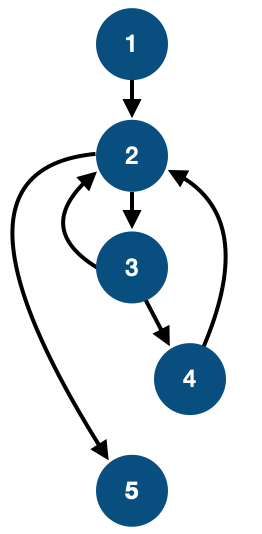
\includegraphics[width=0.35\textwidth]{figures/mccabe.png}
        \label{fig:image:mccabe}
    \end{minipage}
\end{figure}

The function itself is not very complex: it simply counts the number of ``1'' bits in the given integer number. The corresponding graph has 5 nodes and 6 edges. McCabe gives his formula for calculating the complexity from a graph representation as:

\[v~=~e - n + 2p\]

where $v$ is the cyclomatic complexity, $e$ and $n$ represent the number of edges and nodes in the graph, and $p$ is the number of connected components. In this example, $p=1$ and thus $v=3$.

McCabe gives examples of the control graphs for some typical constructs: a \textit{sequence} control, an \textit{if-then-else} control, a \textit{while} control, and an \textit{until} control. Each of the first three are demonstrated in this example: the edge from node 1 to node 2 is a \textit{sequence} control, the edges between nodes 2, 3 and 5 represent a \textit{while} control, and the edges from 3 to 4 and 2 represent an \textit{if-then-else} control.

Thus, the graph nodes correspond to the following lines in the function:

\begin{enumerate}
\item The entry-point of the function at line 1
\item The \texttt{while}-loop at line 4
\item The \texttt{if}-conditional at line 5
\item The ``true'' branch of the conditional at line 6
\item The exit/return from the function at line 10
\end{enumerate}

Measuring the complexity in a consistent way is important when comparing different languages. A tool called \texttt{lizard} was used for all languages except Perl (which was not supported by the tool) and Rust (which exhibited bugs when the data for the Aho-Corasick implementation was reviewed). To gather the metrics for the Perl code a second tool, called \texttt{countperl}, was used. For Rust, a tool called \texttt{rust-code-analysis-cli} from the Mozilla project was used. This tool provided greater depth and detail into the Rust code than \texttt{lizard} had, and did not exhibit the bugs noticed in the data for the Aho-Corasick source code.

It is not clear if the techniques for measuring Perl and Rust were completely identical to the techniques used by \texttt{lizard} for the other languages, so this is noted in the results in section~\ref{subsubsec:complexity}.

\subsubsection{RAPL (Running Average Power Limit)}
\label{subsubsec:rapl}

The \textit{Running Average Power Limit} (RAPL) measurement system was introduced by Intel into their CPU products starting with the Sandybridge family of processors~\cite{khan}. The system allows measuring energy over several areas:

\begin{description}
\item[Package:] The full (socketed) processor package, which may contain multiple cores.
\item[Power-Plane 0:] The domain that encompasses the combined cores within the package. This reading will cover all cores within the CPU of the package.
\item[Power-Plane 1:] Sometimes referred to as ``uncore'', this domain generally covers the integrated GPU (if present).
\item[DRAM:] The domain for the DRAM memory that the CPU is managing, whose energy usage is separate from the package.
\item[Psys:] The domain that covers the entire system-on-chip energy usage. This would include the package and DRAM values, as well as other system-level energy consumption.
\end{description}

A computer system may have more than one package, and the RAPL interface includes methods for determining the number of packages and gathering the energy readings for each package separately. However, it is not possible to measure a package's energy usage at the level of an individual core.

Reading the RAPL data is done through the \textit{model-specific registers} (MSR) interface, as detailed in~\cite[Chapter~14]{intel}. The method involves reading several registers to determine the number of packages the system has, then determining the scaling factors for each of time units (expressed in seconds), power units (Watts), and energy units (Joules). The scaling factors are stored in a single register referred to as \texttt{MSR\_RAPL\_POWER\_UNIT}, as groups of bits within the register. Each scaling factor is a 4-bit (5-bit in the case of energy units) value used to compute a fractional floating-point number (where $b$ represents the value of the n-bit factor):

\[S~=~\frac{1}{2^{b}}\]

In the case of the energy units factor, the value of $b$ on the test platform was 01110b (14), and $S = 61.04~\mu$J.

Obtaining the data during run-time from RAPL required reading from of a series of read-only registers within the MSR and scaling the values obtained by the appropriate value of $S$ for the units. For example, reading the Power-Plane 0 (CPU) energy value uses the \texttt{MSR\_PP0\_ENERGY\_STATUS} register. The value obtained from reading this register is 64 bits in width, though only the initial 32 bits hold energy data (the high 32 bits are reserved by Intel). The value read is masked to remove any high bits, then multiplied by the energy units scale factor to produce a value in Joules.

An issue with the RAPL system was encountered during runs of the experiments: because the value of the energy registers is 32 bits in size, it wraps around to 0 when the maximum value is reached. This caused occasional anomalous readings in cases where the register would reset between the initial reading and the final reading, resulting in a negative overall value. The program that processed the output from the experiments was adjusted to recognize such values and adjust them by applying a constant value computed as $C~=~S \times 2^{32}$, where $S$ is the scaling factor for that value's type (Package, DRAM, etc.).

Adding the appropriate constant for the type of value that was anomalous dealt with the issue and ensured that all iterations of each algorithm and each language would be usable for the analysis of the results.

\subsubsection{Summary of Metrics}

For each execution of a program comprising an experiment, the following data was gathered:

\begin{description}
\item[Total Program Run-time:] The complete run-time of the program, as measured by the harness program. Unlike the next metric, this would include program initialization time, the input/output operations of loading the data to be processed, etc. This is measured in floating-point seconds with micro-second resolution.
\item[Algorithm Run-Time:] The time spent specifically within running the algorithm itself over the complete set of test data. This is measured solely on the processing of data, and does not include I/O, set-up of the environment, or post-algorithm steps such as freeing of memory. Also measured in micro-second resolution.
\item[Maximum Memory Usage:] The largest amount of memory allocated for the running program throughout the course of its execution, in megabytes. This represents the largest size to which the program grew during the run.
\item[Power-Plane 0 (CPU) Energy Usage:] The energy consumed by the CPU cores during the execution of the program. Measured over the full lifespan of the program, not just the algorithm itself. Measured in Joules.
\item[DRAM Energy Usage:] The energy consumed by the DRAM during the full lifespan of the program. Measured in Joules.
\item[Full (Package) Energy Usage:] The energy consumed by the full (socketed) package, which includes the CPU cores' energy but not the DRAM energy. Also measured in Joules.
\end{description}

The Power-Plane 1 (GPU) RAPL values were excluded because the testing machine's package did not have an integrated GPU. Additionally, the Psys values were excluded because they were deemed unnecessary in the context of having the package, CPU and DRAM values.

Independent of the per-program metrics, additional measurements of code expressiveness were made on each of the source files:

\begin{description}
\item[Source Lines Of Code:] The measured lines of code in the implementation of the program, using a tool (\texttt{sloc}) designed to measure these values using consistent standards across the different programming languages.
\item[Cyclomatic Complexity:] The measured complexity of the code, including both the average complexity for the file and specific complexities for those functions that directly correspond to each other across the different implementations.
\item[Conciseness Through Compression:] Using the same tools as were used in the research in~\cite{bergmans} (\texttt{cloc} for removing code comments and \texttt{xz} for data compression), archives of each language's code were compared to each other.
\end{description}

These processes are explained in more detail in section~\ref{subsubsec:conciseness}, along with the results.

\subsection{Experiment Harness}
\label{subsec:harness}

The harness that was developed for managing the execution of the experiment programs was based on the code developed by Pereira, et al~\cite{pereira} and made available via their GitHub repository\footnote{\texttt{\url{https://github.com/greensoftwarelab/Energy-Languages}}}. Their code was adapted and heavily modified to allow for some command-line options controlling features such as the number of iterations each experiment would be run, verbosity of output, etc. It was enhanced to record maximum memory usage and to work with the specific computer selected to be the testing platform.

\subsection{Languages}
\label{subsec:languages}

The languages used were chosen for their commonalities as well as their differences:

\begin{itemize}
\item Three of the languages (C, C++, Rust) are compiled to machine code and were chosen for performance first and foremost. The remaining two (Perl and Python) are interpreted (``scripting'') languages which are highly regarded for speed of development and rapid prototyping, as well as being popular in bioinformatics computing.
\item Each language is currently in widespread use across different disciplines of software development.
\item The languages showcase differing aspects the approach to memory management, as are detailed below.
\end{itemize}

Each language section includes a sample of the language, implementing a naive (O($mn$)) matching algorithm.

\subsubsection{C}

The C programming language is the oldest and most-established of the chosen languages. Originally designed in the early 1970's by Dennis Ritchie, it remains a very widely-used and influential language since its first appearance in 1972. Since 1989, it has been standardized by both ANSI (the American National Standards Institute) and by the International Organization for Standardization (ISO). C was chosen because it is a foundational language in the history of programming languages, and is still in wide use across many fields.

C relies on what is referred to as \textit{manual memory management}, meaning that the programmer is responsible for all allocation and freeing of dynamic memory. This approach can often lead to several major classes of bugs when used incorrectly, such as memory safety issues or memory leaks. Multiple pointers to the same region of memory can become ``dangling pointers'' when one pointer frees the memory without the other pointers being invalidated at the same time. Further attempts to use any of the other pointers can lead to memory corruption or segmentation faults.

Memory management in C is done through a collection of functions in the C standard library, including \texttt{malloc}, \texttt{calloc}, \texttt{realloc}, \texttt{reallocarray}, and \texttt{free}. While \texttt{free} returns allocated memory to the heap, the other functions either allocate memory or change the size of an existing block of allocated memory.

Experiments using the C language were run on three different compiler toolchains: the GNU Compiler Collection (GCC), the LLVM Compiler Infrastructure (LLVM), and the Intel\textregistered~oneAPI Toolkit. This was done to show the subtle differences between programs generated by these compilers, which are free and commonly-used. Due to the low-level nature of C and the maturity of the compilers, C generally performed well at each algorithm compared to other languages. Listing~\ref{lst:naive_c} shows a C implementation of the naive algorithm.

\begin{lstlisting}[language=C,caption={C naive implementation},label={lst:naive_c}]
int match(const char *pattern, const char *string, int **matches) {
  int *saved_matches = NULL;
  int found_matches = 0;
  int m = strlen(pattern);
  int n = strlen(string);

  for (int i = 0; i <= n - m; i++) {
    if (!strncmp((const char *)(string + i), pattern, m)) {
      found_matches++;
      saved_matches = realloc(saved_matches,
                              found_matches * sizeof(int));
      saved_matches[found_matches - 1] = i;
    }
  }

  **matches = saved_matches;
  return found_matches;
}
\end{lstlisting}


\subsubsection{C++}

C++ was developed initially as an extension of C, by Bjarne Stroustrup while working at AT\&T Bell Labs. It first appeared in 1985 and was initially standardized in 1998. At first envisioned as ``C with Classes'', the language has been significantly expanded over the years to include many more features while still maintaining low-level memory accessibility. C++ attempts to offer more expressive, concise coding than C, with many of C's memory-management concerns dealt with automatically by class constructors and destructors. This language was added to the experiments because of its current level of popularity in the sciences, high-performance computing, and other fields. With the addition of C++, it would be possible to compare it directly to C in terms of not just performance but expressiveness and other metrics as well.

In C++, Stroustrup originated the programming idiom of \textit{resource acquisition is initialization}~\cite{cpp} (RAII). Most dynamic memory is managed via class constructors and destructors, though C++ also supports the \texttt{malloc}-based memory management mechanisms inherited from C.

Experiments using the C++ language were also run on the same three compiler toolchains as C: GCC, LLVM, and Intel. Listing~\ref{lst:naive_cpp} shows the naive algorithm implemented in C++.

\begin{lstlisting}[language=C++,caption={C++ naive implementation},label={lst:naive_cpp}]
std::vector<int> match(std::string pattern, std::string string) {
  std::vector<int> matches;
  int m = pattern.length();
  int n = string.length();

  for (int i = 0; i <= n - m; i++) {
    if (pattern == string.substr(i, m))
      matches.push_back(i);
  }

  return matches;
}
\end{lstlisting}


\subsubsection{Perl}

Perl is an interpreted language developed by Larry Wall while working as a programmer at Unisys. The first version, 1.0, was released on December 18, 1987. The current version as of this writing is 5.36.0, released on May 28, 2022.

Perl's reach grew tremendously with the introduction of the World Wide Web's Common Gateway Interface due to its native support for regular expressions and strong text-processing capabilities. Initially developed as a general-purpose scripting language, Perl borrowed features from languages such as C, Awk, Sed, and the \texttt{sh} shell. Perl also offers features generally associated with functional programming, including first-class and higher order functions, lexical closures, garbage collection, and list comprehensions. Perl was chosen for the fact that it has a history with bioinformatics programming that reaches back to the Human Genome Project~\cite{bioperl}, and continues to be popular for rapid development.

Perl is dynamically-typed and multi-paradigm in nature. It supports procedural as well as object-oriented programming styles as well as metaprogramming. Its garbage collection approach to memory management is based on reference counting.

A Perl implementation of the naive algorithm is given in listing~\ref{lst:naive_perl}.

\begin{lstlisting}[language=Perl,caption={Perl naive implementation},label={lst:naive_perl}]
sub match {
    my ($pattern, $string) = @_;

    my $m = length $pattern;
    my $n = length $string;
    my @matches = ();

    for my $i (0 .. ($n - $m)) {
        if ($pattern = substr $string, $i, $m) {
            push @matches, $i;
        }
    }

    return \@matches;
}
\end{lstlisting}


\subsubsection{Python}

Python is another interpreted language, developed by Guido van Rossum while at Centrum Wiskunde \& Informatica in the late 1980's and first released as version 0.9.0 in 1991. Like Perl, it is also dynamically-typed and multi-paradigm in its nature. As a language, Python consistently ranks high in user popularity on such measures as the TIOBE Programming Community Index\footnote{TIOBE Index: \texttt{\url{https://www.tiobe.com/tiobe-index/}}}. Python was added to the list of experiments due to this very high overall popularity, as well as its presence in bioinformatics programming. It is noted for its expressiveness and the ease with which applications can be quickly prototyped.

Python's memory management is a combination of reference counting and a cycle-detecting garbage collector. A Python implementation of the naive algorithm is given in listing~\ref{lst:naive_python}.

\begin{lstlisting}[language=Python,caption={Python naive implementation},label={lst:naive_python}]
def match(pattern, string):
    m = len(pattern)
    n = len(string)
    matches = []

    for i in range(n - m + 1):
        if pattern == string[i:(i + m)]:
            matches.append(i)

    return matches
\end{lstlisting}


\subsubsection{Rust}

Rust is the newest of the languages, having first appeared in 2010. Rust offers a promise of expressiveness with greater safety in the areas of memory management and ownership. It is a multi-paradigm, general-purpose language that draws from several previous languages including C++, Haskell, and Standard ML. While often referred to as a systems programming language, its usage is spreading rapidly to other areas including to some scientific programming disciplines~\cite{nature}. The language began in 2006 as a personal project of Graydon Hoare, an employee of the Mozilla Corporation, with Mozilla beginning to sponsor the work in 2009 and officially announcing the project in 2010~\cite{asay}. The first pre-alpha numbered version of the compiler was Rust 0.1, which was released in January of 2012. The current (as of this writing) version of Rust is 1.65.0 and was released in November of 2022. Rust was chosen in an interest to see how its performance would compare to the other compiled languages (C and C++), and to see in which ways the increased memory safety and other features would contribute to the development process.

An area where Rust is distinct from other C-based languages is in the way it manages memory and tracks values on the stack and heap. Rust uses an ownership system~\cite[Chapter~4]{programming}, with the ability to specify lifetime information for reference types. There is no automated garbage collection, and resources are managed through the same convention of \textit{resource acquisition is initialization} as in C++, with optional reference counting. Rust's design for memory safety does not permit null pointers, dangling pointers, or data races.

With languages such as C and C++, \textit{data ownership} is handled largely through practice and convention. An instance of a C++ \texttt{std::string} owns the buffer allocated for the storage of the string data. Other variables may be created, though, that point to the same buffer or a single character within it. These other interests in the content of the string buffer have their own responsibility for noticing when the original string object is destroyed and the buffer freed. After such point, the outside interests are each responsible for marking their references as no longer valid.

In contrast, Rust integrates the concept of ownership directly into the language itself. Compile-time checks enforce ownership and report violations. When the owner of a value is ``dropped'' (Rust terminology for freeing) the owned value is dropped as well. While the variables themselves are on the stack, the content is allocated on the heap. Variables own their values, and the complex datatypes (structs, tuples, arrays, and vectors) own their elements.

Listing~\ref{lst:naive_rust} shows the naive algorithm as implemented in Rust. Note that the subroutine is named slightly differently in this case, as \texttt{match} is a keyword in Rust.

\begin{lstlisting}[language=Rust,caption={Rust naive implementation},label={lst:naive_rust}]
fn match_string(pattern: &str, string: &str) -> Vec<usize> {
    let mut matches: Vec<int> = Vec::new();
    let m = pattern.len();
    let n = string.len();

    for i in 0..=(n - m) {
        if pattern == string[i..(i + m)] {
            matches.push(i);
        }
    }

    matches
}
\end{lstlisting}


\subsubsection{Languages Not Used}

There were several languages that were considered but ultimately not chosen for the experiments. The Go language is a compiled language growing popularity in data centers. It was set aside in favor of Rust due to the desire to only have one ``young'' language in the set, so as to not distract from the research at hand. The Java language was also considered, but was ultimately not chosen because the additional layer of the Java Virtual Machine might have affected the efforts to gather accurate energy readings. Languages such as C\# that are designed for the .NET framework were passed on over concerns about full Linux usability. Ultimately, it was decided that five languages would be a sufficient set with which to evaluate the chosen metrics and the methodology itself.

\subsection{General Implementation of the Algorithms}

Each of the experiment programs providing an algorithm was implemented according to a consistent structure, to better facilitate the direct comparison of the source code across languages. This structure consists of three basic elements:

\begin{itemize}
\item An ``input'' module that encapsulates the loading of sequence, pattern, and answer data
\item A ``runner'' module that provides the controlling loop of the program
\item An ``algorithm'' module that provides the code specific to the algorithm being used as a basis for the experiment
\end{itemize}

The input and runner modules were written once per language and re-used across all algorithms.

\subsubsection{Input modules}

The input modules allow the main-loop modules (described next) to further abstract the reading of the external data used in each experiment. Data is separated into three files: the \textit{sequences} file contains lines of randomly-generated target strings, the \textit{patterns} file contains the crafted patterns to search for within the sequences, and the \textit{answers} file provides a representation of the correct number of times each pattern should be found in each sequence. This allows the runner modules to verify the results of each invocation of the algorithms being evaluated. The nature of the data and its creation is further detailed in~\ref{subsec:data}.

Each input module defines three routines, one for each of the data files. In most cases, the reading of the pattern files was essentially identical to the sequence files and thus the pattern routine simply calls the sequence routine.

The input modules are the first place in which the distinction in expressiveness and style between the languages becomes apparent. Differences become immediately visible in just the comparison of the C and C++ implementations, where the physical combined length of files (in C and C++, the input modules also required accompanying header files) differs by over 40\% in favor of C++. Python measures as being just over 20\% of the size of the C code.

\subsubsection{Runner modules}

Each runner module utilizes the input module to read in the experiment data and loop over it. In the single-pattern algorithms (which includes the approximate-matching algorithm), this is a nesting of two loops: the outer loop iterates over the set of pattern strings and the inner loop iterates over the set of sequence strings. Each iteration of the loop over the sequence strings triggers one execution of the algorithm being evaluated. In the multi-pattern algorithms, this is a single loop over the set of sequence strings, as the complete set of patterns are pre-processed prior to the loop.

The runner records the time according to the system wall-clock when the algorithm pre-processing begins, and the time when all loops and answer validation has completed. Everything that is not input-related or related to reporting of results is recorded in this span of time. At this point, the runner prints three lines to the standard-output stream. The lines identify the language (including compiler variants for C and C++), the algorithm, and report the time spent in the main loop. The runner is also responsible for handling the arguments passed to the program as well as determining the exit-code of the program (to allow the harness program to discern failing runs from successful runs).

\subsubsection{Algorithm modules}

The algorithm modules are at the heart of the experiments. To maintain consistency, each algorithm module defines a minimum of two functions: an initialization routine and the primary algorithm entry point.

The initialization routine is responsible for any pre-processing necessary for the pattern string, and produces a collection of data elements that represent the pattern in the appropriate internal structure. The exact nature and structure of this representation is language-dependent as well as algorithm-dependent.

The algorithm entry point routine is the means by which each algorithm was applied to the pattern and sequence under consideration. It receives the pattern representation produced by the initialization routine and the sequence representation as parameters, and returns a numerical value indicating how many times the pattern was successfully found within the sequence. In the case of the multi-pattern algorithm implementation, the return value from this routine is a vector of numbers with length equal to the number of patterns.

In addition to these two functions, each algorithm module defines all needed support code for the initialization and entry point. In some cases (such as the C and Rust implementations of the Aho-Corasick algorithm) this included minimal implementations of data structures such as sets and simple queues.

Each algorithm module also provides the language-specific equivalent of a ``main'' function, that function which is treated as the program entry-point by the operating system. Each ``main'' function consists of a single call to the runner function provided by the runner module. The call passes the two algorithm-specific functions as pointers (again, in a language-dependent manner) to the runner, followed by the name of the algorithm and a representation of the command-line arguments.

\subsection{Algorithm Implementation Details}

The different algorithms that were chosen are listed here in the order of their implementation. Each of the algorithms was implemented first in C, as a baseline. These C implementations were then used as templates for the other languages' implementations. In addition to helping to keep the implementations approximately similar and equal, this provided insight into the differences that the features and expressiveness of the different languages made in the development process itself.

Any inefficiencies observed in the experiments' implementations are due to this decision.

\subsubsection{Knuth, Morris, and Pratt}

The C implementation of Knuth-Morris-Pratt was adapted from~\cite[Chapter 7]{handbook}. Of note is the discovery that the sample code quietly takes advantage of C's use of a ``null'' byte at the end of a string to stand in for the sentinel character that the algorithm appends to the pattern string. While this optimization was also applicable to C++ (where strings are represented by instances of the \texttt{std::string} class), each of the three remaining languages were required to manually add a sentinel character to each pattern string prior to computing the corresponding ``next'' table.

This being the first of the algorithms implemented, it is also where the means of passing generic data from the initialization routines to the algorithm routines was developed. The differences in these methods, particularly between the compiled languages, spoke strongly to their relative expressiveness.

In the C implementation it was necessary to use a memory pointer of the type, \texttt{void~**}. This defines a dynamic list of dynamic pointers, but provides no information about each individual pointer. It is left to the code to properly type-cast the values from this block of memory. If the program is incorrect (such as getting the order of elements wrong) the resulting typed pointers will likely trigger memory faults when dereferenced. This was also the most-flexible of the compiled solutions and required no difference in implementation between the different algorithms.

In C++ it was initially attempted to reuse the \texttt{void~**} approach that had been used in C. This proved to be extremely difficult under the stricter compiler rules, and the decision was made to use the \texttt{std::variant} class instead, which represents a type-safe union in the C++ language. While the same variant type definition could have been used for both the single-pattern and multi-pattern algorithms, it was decided to distinguish them for the sake of readability. The type definitions were made in the file \texttt{run.hpp}, the header-file for the runner module of C++. Unpacking a vector of the variant types brought further type-safety in the form of a generically-typed function \texttt{get<>} in the standard library that was used to extract the values to new objects of the correct type.

Rust had the language features that seemed the most clear and expressive in implementation: enumeration and pattern-matching. In Rust, an enumeration type (\texttt{enum}) can optionally assign data types to the elements of the enumeration. When an enumeration element is instantiated it is provided an instance of that data when applicable. This lead to a system for the Rust programs in which the initialization function for an algorithm created and returned a vector of the enumeration type. The algorithm routines that received these types would extract them from the vector using a pattern-matching\footnote{In the computer language sense, not to be confused with pattern-matching in strings.} construct that ensured the types of each individual element of the vector received from the initialization function. The program would raise a run-time exception if the given vector element was not of the expected type. In contrast, Rust required the least-expressive approach to appending the sentinel value onto the pattern string for the sake of creating the ``next'' table.

Given the dynamically-typed nature of data in Perl and Python, both of these implementations were simple lists of values returned without any extra effort at encoding. As with the \texttt{void~**} approach the onus was on the program to unpack the elements in the correct order. Trying to use a list or list-reference value as an ordinary scalar value would have caused a run-time exception in either language.

\subsubsection{Boyer and Moore}

The C version of the basic algorithm was drawn from~\cite[Chapter 14]{handbook}. Like Knuth-Morris-Pratt, it requires a character at the end of the pattern for calculating the suffixes table. The C and C++ implementations used the ``null'' string-terminating byte for this while the others added it explicitly.

Starting the analysis with Rust in this case, one aspect became very clear in this algorithm's implementation: the need to regularly cast various numerical (particularly integer) types to other types. Because of the larger amount of array-indexing in this algorithm, the number of times an \texttt{i32} (signed 32-bit integer) or \texttt{u32} (unsigned) had to be cast to or from a \texttt{usize} type (an unsigned type used for lengths and indexing) was significant. While this does lead to fewer bugs in the code, at the same time it detracted from the conciseness and readability of the Rust version.

Perl and Python were comparable in their conciseness and logical expression of this algorithm. Python showed an advantage in the form of its native support for iterators as a type and functions such as \texttt{range} that return these iterators. Operations like looping backwards through a series of integers was clearer in the Python code than in the corresponding Perl.

The C and C++ implementations are best compared to each other, as this is another case where the C++ Standard Library classes lead to clearer code. Though there was less difference in code-length, various mechanisms of C++ in areas such as argument-passing meant less overhead and less ambiguity about pointers sent and received.

\subsubsection{Bitap}

The C version of Bitap was taken from~\cite[Chapter 5]{handbook}, where it is referred to as Shift-Or. The design of the algorithm given there is clearly drawn from the Shift-Or algorithm illustrated in~\cite{baeza}. The C++ version followed the C very closely with the only changes being the use of the C++ standard classes for strings and vectors. Likewise, the Rust version of this algorithm proved very simple and bore a reasonable resemblance to the C and C++.

\begin{lstlisting}[language=Rust,caption={Bitap main loop in Rust},label={lst:bitap_rust}]
for j in 0..n {
    state = (state << 1) | s_positions[sequence[j] as usize];
    if state < *lim {
        matches += 1;
    }
}
\end{lstlisting}


The Perl and Python implementations were also very similar to the compiled versions, with the same exception that each language has arrays as first-class data types. The Python version, however, did have one notable difference: due to Python's integers being of arbitrary size, it was not enough to take the bit-complement of 0 to get a ``full'' bit-field. In Python this resulted in a value of -1, rather than the expected $2^W - 1$ (where $W$ is the word-size used within the algorithm). To force Python to treat these values as unsigned 64-bit, it was necessary to declare a ``mask'' value equal to $2^W - 1$ and apply this to the result of every logical bit-operation performed. This incurred a significant performance penalty on the Python implementation, giving it the widest performance gap when compared against its Perl counterpart.

\subsubsection{Aho and Corasick}

For the implementation of this algorithm, no existing code was consulted. Rather, the initial C version was developed directly from the algorithm specification in the paper itself. The C version required the most supporting code, as the algorithm calls for both queue and set data structures. Additionally, the construction of the $g$ and $output$ functions required dynamic re-sizing of lists. It was chosen to avoid this added complexity by generously estimating the size needed for those lists and pre-allocating that amount. Constructing $f$ did not have this problem as the size was known at that point from having created the previous arrays. Both queue and set data structures were implemented with just the minimally-required functionality for each. For the queue, this was the operations \textit{create}, \textit{delete}, \textit{expand} (grow), \textit{enqueue}, \textit{dequeue}, and a test for whether the queue is empty. For the set, these were \textit{insert}, \textit{test-for-membership}, and an implementation of a \textit{union} operation. The set's structure was designed in a such a way that using the C \texttt{calloc} function was sufficient for both creation and initialization, and \texttt{free} was sufficient for deletion and clean-up. That said, these implementations did add to the number of dynamic memory allocations and corresponding releases.

When implementing in C++, the C++ Standard Library was able to provide existing classes for both set and queue implementations, greatly reducing the amount of supporting code in this version. Though C++ vector types can dynamically grow, intermediate experiments found that relying on this for the $g$ and $output$ function construction introduced a slight performance penalty. As such, it was decided to replicate the C approach of estimating the size of $g$ and $output$ and pre-allocating. Using C++ features, this also allowed for immediate initialization of the vectors where the C arrays required explicit loops to initialize. In the end, the difference between the two languages' implementations was a factor of almost 2x in SLOC for the C code over the C++ code.

The Perl and Python implementations were both significantly shorter in length than the C or C++, due largely to native support for resizable lists. For the queue data structure, the Python code used the \texttt{collections.deque} class that is part of the Python core. Perl used an ordinary list, as the language provides a built-in keyword for removing from the head of a list in O(1) time. Both languages grew the $g$ and $output$ functions dynamically rather than pre-allocating them. For the implementation of a set data structure, Python provides a \texttt{set} type as a native data type. The Perl version initially used the native associative array type, a common technique for emulating sets in Perl. This proved to be a slight performance penalty, so it was later replaced with a simple list of integers that had duplicates removed as needed.

Lastly, the Rust implementation went through several iterations before reaching its final form. The first version closely followed the C++ version: the use of resizable vectors through the native \texttt{Vec<>} type, and implementations of set and queue from the standard Rust library (\texttt{std::collections::HashSet} and \texttt{std::collections::VecDeque}, respectively). This initial version severely under-performed in comparison to the other two compiled languages. With help from the Rust community, it was determined that the two collection classes were incurring large amounts of overhead. To address this, they were replaced with simple implementations adapted from the C code. As with the Perl and Python versions, the \texttt{Vec<>} type was allowed to handle the dynamic nature of the $g$ and $output$ functions. As with C++, some intermediate experiments were performed that pre-allocated these vectors based on estimates of needed space. But unlike with C++, it was found that at best the performance remained the same, and in some runs was noticeably worse. As a result, the pre-allocation was removed.

\subsubsection{Approximate Matching by DFA with Gaps}

As this algorithm was new material, it was difficult to anticipate what concerns and issues would arise. Some aspects of each implementation were close in design to the Aho-Corasick code due to the fact that both algorithms are centered around a DFA. All implementations were based on the developed algorithms~\ref{alg:create_dfa} and~\ref{alg:find_pattern_with_gaps}, from section~\ref{subsec:dfa_gap}.

\begin{lstlisting}[language=C,caption={C/C++ DFA-Gap main loop},label={lst:dfa_c}]
for (int i = 0; i <= end; i++) {
  int state = 0;
  int ch = 0;
  while ((i + ch) < n && dfa[state][sequence[i + ch]] != FAIL)
    state = dfa[state][sequence[i + ch++]];

  if (state == terminal)
    matches++;
}
\end{lstlisting}


As was the case with some of the previous algorithms, the main differences between the C and C++ implementations were in the use of C++ standard library classes in place of manual memory management; their main loops were identical (listing~\ref{lst:dfa_c}). The availability of a postfix-increment operator in these languages allowed the two statements of lines 8--9 in algorithm~\ref{alg:find_pattern_with_gaps} to be combined into a single statement. Unlike the Aho-Corasick DFA allocation, this algorithm has a predictable number of states. This made allocation of the DFA much more exact and clean in comparison.

The Rust version of this algorithm is largely identical in structure to the C and C++ versions. In terms of SLOC, it comes in longer than either of those, due primarily to the number of lines used for pattern-matching in the processing of the pattern data structure created by the initialization routine.

The Perl implementation suffered from some readability issues attributable to the ways in which Perl handles slicing arrays that have been passed by reference rather than by value. Perl also features a postfix-increment operator, allowing a savings of one line in the SLOC score. In contrast, the Python implementation once again gained conciseness and readability through its clear syntax around iterators and slightly cleaner syntax around treating strings as arrays and applying slicing operations to them.

\subsubsection{Regular Expressions Variant}
\label{subsubsec:dfa_regexp}

The performance of the Perl and Python languages on the DFA-Gap algorithm led to some critical thinking about how this algorithm might actually be implemented in those languages in a real application. This, in turn, led to an extra experiment being written for each of these two languages.

Both Perl and Python have native support for extended regular expressions as a part of the language. When this is taken into account, it is found to be preferable to use the implementation of the DFA as a regular expression. The regular expression engines in both Perl and Python are implemented in compiled code and are thus much faster than the hand-coded DFA implementations.

As will be shown in section~\ref{subsubsec:results:perf_perl_python}, this had a very significant effect on the overall performance of the gap algorithm for those two languages.

The key to meeting the four requirements in section~\ref{subsec:regexp_variant}, particularly the fourth requirement, was a mechanism called \textit{positive-lookahead}. This mechanism allows the engine to match the pattern as a sequence ahead of the current point, without actually consuming any of the matched characters. This was instrumental in finding overlapping matches.

Once this had been undertaken in Python and Perl, it was necessary to implement similar experiments for the compiled languages. In the case of C++, a class for regular expressions had been part of the C++ Standard Library since the adoption of the C++11 standard. C, as well, offered regular expression support in the form of the POSIX regular expressions functions included as part of the C standard library. Rust, though, did not have built-in regular expression support.

It was decided to use the \texttt{regex} ``crate''\footnote{A ``crate'' is the term used in the Rust community for a packaged library or extension.} that was available for Rust, while using the native regular expression support in C and C++. This exposed problems: The C and C++ engines proved to be exceedingly slow, and unable to properly identify the matched substrings. Additionally, Rust's \texttt{regex} package did not support the positive-lookahead feature of regular expressions that was necessary to prevent making multiple passes over the target string.

The solution came in the form of the Perl-Compatible Regular Expressions engine. As the name hints, the engine provides support for the various extensions to regular expression syntax introduced by Perl (as well as other languages and dialects). In particular, PCRE supports both positive-lookahead and capturing within the lookahead. Lastly, while written for the C language it was possible to use this engine in both C++ and Rust through wrapper libraries.

As the results will show, the effectiveness of regular expressions varied across the languages.

\subsection{Initial Observations on Complexity}

At this point, some initial observations could be made about the complexity measurements of some of the code. In the code examples given throughout section~\ref{subsec:languages}, all implementations of the naive algorithm had the same cyclomatic complexity value of 3. All also produced the same directed flow graph, shown in figure~\ref{fig:graph-naive}. In this graph, nodes 1 and 6 represent the entry and exit to the function. Node 2 represents the for-loop, and node 3 represents the if-else conditional block.

\begin{figure}[ht]
    \centering
    \begin{tikzpicture}[shorten >=1pt,node distance=1.5cm,on grid,auto]
    \node[state] (s_1)                {1};
    \node[state] (s_2) [below of=s_1] {2};
    \node[state] (s_3) [below of=s_2] {3};
    \node[state] (s_4) [right of=s_3] {4};
    \node[state] (s_5) [below of=s_3] {5};
    \node[state] (s_6) [below of=s_5] {6};

    \path[->]
        (s_1) edge             node {} (s_2)
        (s_2) edge             node {} (s_3)
        (s_2) edge[bend right] node {} (s_6)
        (s_3) edge             node {} (s_4)
        (s_3) edge             node {} (s_5)
        (s_4) edge             node {} (s_5)
        (s_5) edge[bend left]  node {} (s_3);
\end{tikzpicture}


    \caption{Flow graph of the naive algorithm}
    \label{fig:graph-naive}
\end{figure}

Part of the reason for this is that the complexity measurement does not take into account calls to functions. This is by intent, as factoring out content to a separate function is part of the process of managing complexity. In the cases of C and C++, both utilized library functions: \texttt{strncmp} in C and \texttt{substr} in C++. In contrast, the use of \texttt{substr} in Perl is a keyword of the language. Python and Rust skip this entirely by virtue of having array-slicing be a core language feature, along with the ability to compare slices directly. Had the complexity-measuring tools taken the library calls into account, that would have changed the graph for those languages from one connected component to two, and resulted in a higher overall complexity score.

Compare this to the \texttt{make\_next\_table} functions defined in the implementations of Knuth-Morris-Pratt. The complexity tool found the Python version to have a score of 6 while the C and C++ versions both scored 5. The reason for the distinction is that C and C++ allocated the array variable \textit{next\_table} prior to the function call and passed it as a parameter. By contrast, in Python \textit{next\_table} was created within the function. The loop used to create it is the source of the extra point of complexity. Figures~\ref{fig:graph-kmp-py} and~\ref{fig:graph-kmp-cpp} illustrate these slightly-different flow graphs. In figure~\ref{fig:graph-kmp-py}, states 2 and 3 represent the extra for-loop that introduces the extra point of complexity.

\begin{figure}[ht]
    \centering
    \begin{minipage}[t]{0.45\textwidth}
        \centering
        \begin{tikzpicture}[shorten >=1pt,node distance=1.5cm,on grid,auto]
    \node[state] (s_1)                 {1};
    \node[state] (s_2)  [below of=s_1] {2};
    \node[state] (s_3)  [below of=s_2] {3};
    \node[state] (s_4)  [below of=s_3] {4};
    \node[state] (s_5)  [below of=s_4] {5};
    \node[state] (s_6)  [below of=s_5] {6};
    \node[state] (s_7)  [below of=s_6] {7};
    \node[state] (s_8)  [right of=s_7] {8};
    \node[state] (s_9)  [below of=s_7] {9};
    \node[state] (s_10) [below of=s_9] {10};

    \path[->]
        (s_1) edge             node {} (s_2)
        (s_2) edge             node {} (s_3)
        (s_2) edge[bend right] node {} (s_4)
        (s_3) edge[bend right] node {} (s_2)
        (s_4) edge             node {} (s_5)
        (s_4) edge[bend right] node {} (s_10)
        (s_5) edge             node {} (s_6)
        (s_5) edge[bend right] node {} (s_7)
        (s_6) edge[bend right] node {} (s_5)
        (s_7) edge             node {} (s_8)
        (s_7) edge             node {} (s_9)
        (s_8) edge[bend right] node {} (s_5)
        (s_9) edge[bend left]  node {} (s_5);
\end{tikzpicture}


        \caption{Flow of the Python \texttt{make\_next\_table} function}
        \label{fig:graph-kmp-py}
    \end{minipage}\hfill
    \begin{minipage}[t]{0.45\textwidth}
        \centering
        \begin{tikzpicture}[shorten >=1pt,node distance=1.5cm,on grid,auto]
    \node[state] (s_1)                {1};
    \node[state] (s_2) [below of=s_1] {2};
    \node[state] (s_3) [below of=s_2] {3};
    \node[state] (s_4) [below of=s_3] {4};
    \node[state] (s_5) [below of=s_4] {5};
    \node[state] (s_6) [right of=s_5] {6};
    \node[state] (s_7) [below of=s_5] {7};
    \node[state] (s_8) [below of=s_7] {8};

    \path[->]
        (s_1) edge             node {} (s_2)
        (s_2) edge             node {} (s_3)
        (s_2) edge[bend right] node {} (s_8)
        (s_3) edge             node {} (s_4)
        (s_3) edge[bend right] node {} (s_5)
        (s_4) edge[bend right] node {} (s_3)
        (s_5) edge             node {} (s_6)
        (s_5) edge             node {} (s_7)
        (s_6) edge[bend right] node {} (s_3)
        (s_7) edge[bend left]  node {} (s_3);
\end{tikzpicture}


        \caption{Flow of the C++ \texttt{make\_next\_table} function}
        \label{fig:graph-kmp-cpp}
    \end{minipage}
\end{figure}

The resulting complexity of the various implementations is explored in more depth in section~\ref{subsubsec:complexity}.

\subsection{Optimizations}

Over the course of the development of the experiments in each language, the need became clear for some basic optimizations. In every case, any optimization was applied consistently across all languages. Some examples of optimizations include:

\begin{description}
\item[Data Preprocessing:] While the C and C++ languages were able to seamlessly use individual characters from the strings as array indices, Rust and the interpreted languages were not. Based on an assumption that production-targeted code would apply any similar preprocessing, the strings were converted to forms directly usable by the other languages. In the case of Rust, this was a conversion of strings to arrays of unsigned 8-bit integers. In the case of Python, it was a direct mapping of strings (which are already treated as sequences by Python) into the ordinal values of each character. Perl required the most preprocessing, with strings first being converted to arrays of individual characters before being mapped to their ordinal values.
\item[Pattern Preprocessing:] To bring down the running times of the interpreted languages' experiments, a mechanism for preprocessing patterns was developed that allowed for each pattern to be processed only once prior to being applied to all sequences. Without this, some instances of the Knuth-Morris-Pratt algorithm (for example) took close to an hour to complete. Once the structure of this was established, it was also applied to the compiled languages as well.
\item[Minimizing Type-Casting:] In the case of Rust's strong typing, it was necessary to frequently cast integer values into Rust's \texttt{usize} type for use as array indices. Though this would have had little or no effect on run-time, the decision was made in some cases to declare a cast version of the integer value to help in the overall readability of the code.
\item[Compiler Options:] For the three compiled languages, consistent choices of compiler options for optimization were applied. For the C and C++ code, the same options were used for both languages. For the Rust code, the \texttt{cargo} utility was run with an option that instructed the compiler to build optimized code instead of debug-instrumented code. These were not applicable to the Perl and Python code, as both of those are interpreted languages.
\end{description}

All code-optimization steps were designed to be done inside the timing window of the runner module, and contributed to the reported algorithm run-time.

\subsection{Experimental Data}
\label{subsec:data}

The data used for the experiments was generated in a random fashion. It was specifically created to emulate basic DNA data, while keeping the size of the data manageable from the perspective of the programs that would be run.

\subsubsection{Method of Generation}

Data generation was handled by a Python script written to allow almost all parameters of the resulting data to be tuned. The script's options included a seed value for the random number generator, which allowed for consistent generation of the data once the parameters were tuned to satisfaction.

Sequence generation was a straightforward process of determining a length from the provided base length and variance values. The standard random number generator provided by Python was then used to draw the sequence of $n$ letters from the set of valid characters.

To ensure that algorithms would be as thoroughly exercised as possible, each candidate pattern was tested before acceptance. The requirement for acceptance was that it match a minimum threshold (0.10\%) of the full set of sequences. Generation of the patterns was done by first selecting the pattern length from the specified range, then extracting a sequence of that length from a random location in a candidate sequence. Candidate sequences were chosen by selecting every $i^{th}$ sequence from the full list (starting with the first sequence), with $i$ being the total number of sequences divided by the total number of patterns being generated.

For the approximate-matching algorithm, the same set of patterns was used since they were already known to meet the minimum-matching criteria. For this algorithm, a $k$ value of 0 would lead to the same set of matches as an exact-matching algorithm would find.

\subsubsection{Shape of the Data Used}

The data set selected for these experiments consisted of the following:

\begin{itemize}
\item 100,000 sequence strings of length ranging from 1,008 to 1,040 characters ($1,024 \pm 16$). The number of patterns and their length was chosen to provide sufficient data to extensively exercise each algorithm implementation.
\item 100 pattern strings of length ranging from 8 to 10 characters ($9 \pm 1$). The length was adjusted several times through command-line parameters to the data-generation utility until a size was found for which the generated patterns would reliably meet the minimum threshold for sequences matched. The matching percentage over the 100 patterns ranged from 0.10\% to 1.62\%, with an average of 0.76\%.
\item A full set of correct counts of each pattern's occurrences in each sequence, as would be found by an exact-matching algorithm. This was established using a backtracking regular expression search for each of the selected patterns over each of the generated sequences. The regular expression was designed to properly include overlapping pattern occurrences.
\item An additional set of answer-files were generated for the approximate-matching algorithm, for values of $k$ ranging from 1 to 5. These, too, were generated using crafted regular expressions that would detect overlapping occurrences of the patterns.
\end{itemize}

A smaller data set was also generated for the purpose of testing and validation of the programs prior to full experiment runs.

The size of the data set was chosen after some preliminary experiments showed this size to be large-enough to rigorously exercise the algorithms while still running in reasonable time overall. This allowed for the experiments to be run repeatedly as the code itself evolved.

\subsection{Testing Platform}
\label{subsec:testing_platform}

The experiments were run on a dedicated machine running a version of the Linux operating system. The set of installed software was kept minimal to reduce the chance of background processes influencing the readings of general energy usage during the runs of experiments.

\subsubsection{Hardware Specifications}

The machine used for the experiments was an Intel-brand NUC7i5BNH i5-7260U, an ultra-compact device referred to by Intel as a ``Next Unit of Computing'' (NUC). The machine features the following specifications:

\begin{table}[h!]
\begin{center}
\begin{tabular}{|ll|}
\hline
Processor & Intel\textregistered~Core\texttrademark~i5-7260U Processor\\
Processor Base Frequency & 2.20 GHz\\
Max Turbo Frequency & 3.40 GHz\\
Memory Type & DDR4-2133 1.2V SO-DIMM\\
Installed Memory & 8 GB\\
Internal Drive Form Factor & M.2 and 2.5''\\
Installed Storage & 120 GB M.2 SSD\\
\hline
\end{tabular}

\caption{Hardware specifications of the test platform}
\end{center}
\label{table:hardware_specs}
\end{table}

The CPU is dual-core, with hyperthreading cores, for a total of 4 computational cores. This did not affect the experiments as none of the code was written to be multi-threaded.

\subsubsection{Operating System and Configuration}

The NUC was cleaned of the vendor-installed operating system. Linux was installed on it using the minimal server edition of Ubuntu Linux 22.04.1. All unnecessary packages and software services were either disabled or removed completely.

The development software (see next section) was then installed. This included the Linux version of the ``Homebrew'' package manager. Homebrew was specifically used to install the latest version of the LLVM Compiler Infrastructure, to allow all experiment code to be compiled directly on the NUC (rather than copying executable files built on a different machine). The Python and Perl interpreters that were used were also provided by Homebrew, as were the majority of the tools used for developing, testing, and evaluating the experiments on the development platform. The Rust language toolchain was installed and managed using the ``Rustup'' management software. Core software development packages from Ubuntu were also installed at this time.

\subsubsection{Compilers and Other Tools}

Table~\ref{table:software_specs} lists the primary software tools and packages that were used in the creation and execution of the experiments, with the source from which they were obtained. The double line after the Python details indicates that the remaining tools were used on the development machine only, not on the experiments platform. These tools were used in the testing and evaluation of the experiments code separately from running experiments on the NUC.

\begin{table}[h!]
\begin{center}
\begin{tabular}{|l|r|l|}
\hline
\textbf{Tool} & \textbf{Version} & \textbf{Source}\\
\hline
GNU Make & 4.3 & Ubuntu 22.04\\
GCC & 11.2.0 & Ubuntu 22.04\\
LLVM & 15.0.3 & Homebrew\\
Intel\textregistered~oneAPI Compiler & 2022.2.0 & Intel\\
Rust & 1.64.0 & Rustup Manager\\
Perl & 5.36.0 & Homebrew\\
Python & 3.10.8 & Homebrew\\
\hline
\hline
Valgrind & 3.20.0 & Homebrew\\
\texttt{sloc} & 0.2.1 & Homebrew\\
\texttt{perf} & 5.15.53 & Ubuntu 22.04\\
\texttt{cloc} & 1.94 & Homebrew \\
\texttt{xz} & 5.2.7 & Homebrew \\
\texttt{lizard} & 1.17.10 & Homebrew \\
\texttt{countperl} & 1.0.1 & Ubuntu 22.04 \\
\hline
\end{tabular}

\caption{Specifications of software tools used}
\label{table:software_specs}
\end{center}
\end{table}

The tools used for the experiments themselves do include the GNU Make tool, as it was the driver for automating the running of the full range of experiments on a regular basis.

\subsection{Resources}

All source code for all experiment programs, as well as the harness utility described and the Python utilities used for data generation and processing of results, is available on the GitHub platform~\cite{github}.
